\documentclass[tikz,border=2pt]{standalone}
\usepackage{amsmath}
\usepackage{pgfplots}
\pgfplotsset{compat=1.18}
\usetikzlibrary{arrows.meta}
\begin{document}
% IPV with n = 2 and theta_i ~ U[0,1]: a strategy is a bidding function of the valuation.
% Second-price equilibrium b(theta) = theta, first-price equilibrium b(theta) = theta/2;
% the type theta_1 = 0.7 bids 0.7 and 0.35 respectively.
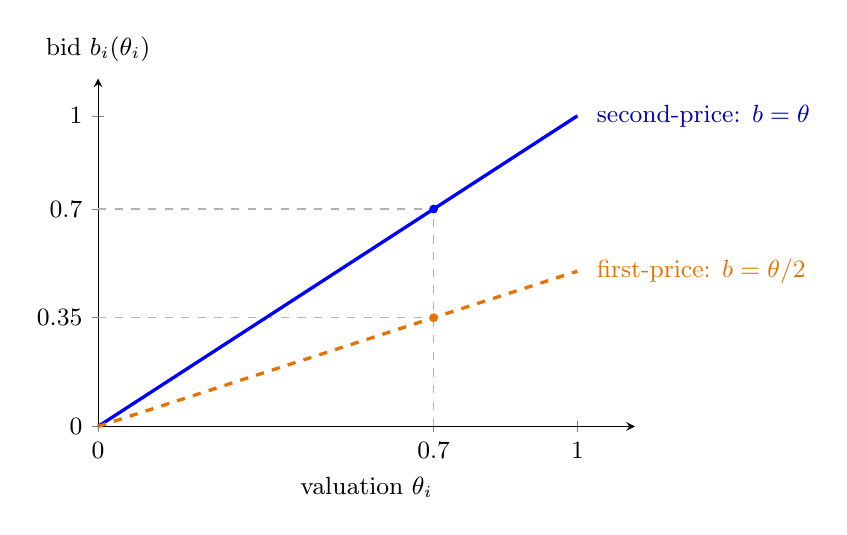
\begin{tikzpicture}[font=\small, >={Latex[length=2mm]}]
  \begin{axis}[
    axis lines=left, xmin=0, xmax=1.12, ymin=0, ymax=1.12,
    xtick={0,0.7,1}, ytick={0,0.35,0.7,1},
    xticklabels={$0$,$0.7$,$1$}, yticklabels={$0$,$0.35$,$0.7$,$1$},
    xlabel={valuation $\theta_i$}, ylabel={bid $b_i(\theta_i)$},
    ylabel style={rotate=-90, anchor=south, at={(axis description cs:0,1.02)}},
    width=8.4cm, height=6cm, clip=false]
    \addplot[gray!60, thin, dashed] coordinates {(0.7,0) (0.7,0.7)};
    \addplot[gray!60, thin, dashed] coordinates {(0,0.7) (0.7,0.7)};
    \addplot[gray!60, thin, dashed] coordinates {(0,0.35) (0.7,0.35)};
    \addplot[blue, very thick, domain=0:1, samples=2] {x};
    \addplot[orange!90!black, very thick, dashed, domain=0:1, samples=2] {x/2};
    \fill[blue] (axis cs:0.7,0.7) circle (1.6pt);
    \fill[orange!90!black] (axis cs:0.7,0.35) circle (1.6pt);
    \node[blue!70!black, anchor=west] at (axis cs:1.02,1) {second-price: $b=\theta$};
    \node[orange!90!black, anchor=west] at (axis cs:1.02,0.5) {first-price: $b=\theta/2$};
  \end{axis}
\end{tikzpicture}
\end{document}
